%!TEX TS-program = xelatex
%!TEX encoding = UTF-8 Unicode

\documentclass[12pt,a4paper]{article}
\usepackage{fontspec,xltxtra,xunicode}
\usepackage{fancyhdr}
\usepackage[a4paper,margin=3cm]{geometry}
\setmainfont[Scale=1.22]{TH Sarabun New}
\XeTeXlinebreaklocale 'th_TH'

% Source code
\usepackage{listings}
\lstdefinestyle{sitdhcodelisting}{
    frame=trBL,
    label=trianglecheck,
    showspaces=false,
    numberstyle=\tiny, 
    language=Java, 
    numbers=left,   
    firstline=1
}

% Graphic
\usepackage{graphicx}
% Multiple row
\usepackage{multirow}

\newcommand{\sitdhibong}{สิทธิพงษ์ เหล่าโก้ก}
\newcommand{\studentid}{5870972621}
\newcommand{\department}{สาขาวิชาวิศวกรรมซอฟต์แวร์}
\newcommand{\faculty}{คณะวิศวกรรมศาสตร์}
\newcommand{\myprogram}{แผน ข. ภาคนอกเวลาราชการ}
\newcommand{\university}{จุฬาลงกรณ์มหาวิทยาลัย}
\newcommand{\subject}{Software Testing and Quality Assurance}

\renewcommand{\lstlistingname}{รายการที่}
\renewcommand{\figurename}{ภาพที่}

\pagestyle{fancy}
\lhead{\subject}
\rhead{การบ้านครั้งที่ 4: Path testing}
\lfoot{\sitdhibong: \studentid}

% Source code cosmatic
\lstset{columns=fullflexible,basicstyle=\ttfamily}

\begin{document}
% Triangle check
\section{โปรแกรมคำนวณรูปสามเหลี่ยม}
\label{listing:trianglecal}
จากรายการความต้องการเพื่อตรวจสอบรูปสามเหลี่ยม จะนำมาเขียนโปรแกรมด้วยภาษา JavaScript ดังแสดงให้เห็นด้านล่าง
\lstinputlisting[style=sitdhcodelisting, title=\lstname, caption=โปรแกรมตรวจสอบรูปสามเหลี่ยมภาษา JavaScript]{src/compute.js}

\newpage
% Control flow graph
\section{Control flow graph}
จากโปรแกรมคำนวณรูปสามเหลี่ยมจาก \lstlistingname\, \ref{listing:trianglecal} นำมาวาด Control flow graph ได้ดังรูปด้านล่าง

\begin{figure}[h!]
    \label{fig:flowgraph}
    \centering
    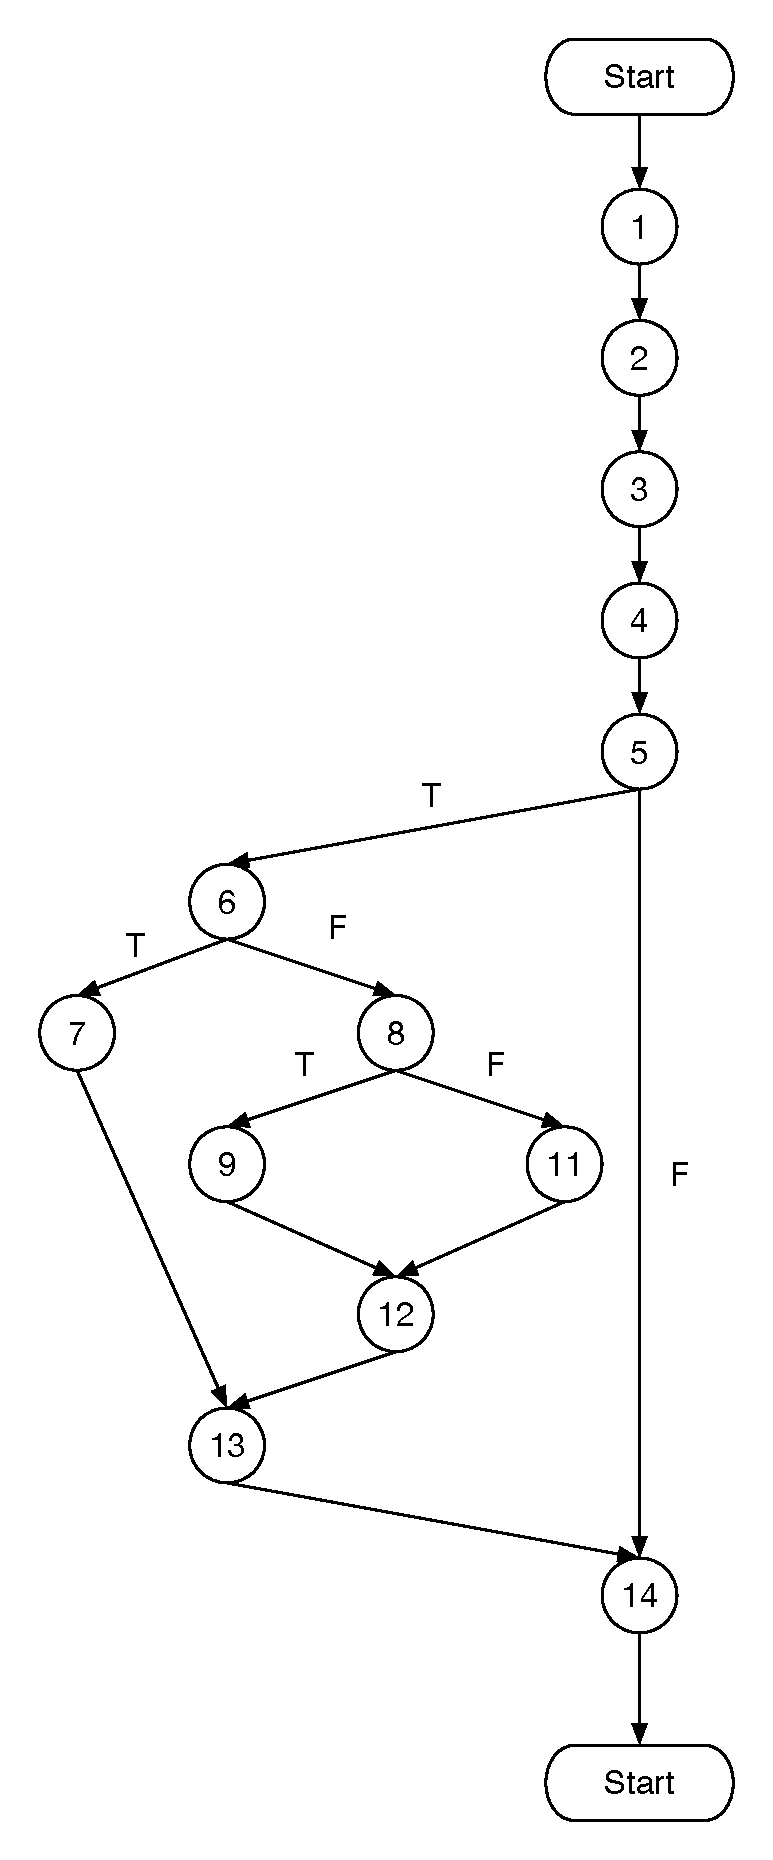
\includegraphics[height=0.8\textheight]{img/graph-testing.eps}
    \caption{Control flow graph ของโปรแกรมตรวจสอบรูปสามเหลี่ยมจาก \lstlistingname\, \ref{listing:trianglecal}}
\end{figure}

\newpage
% Coverage table
\section{Coverage table}

% ID, Path, Decisionx3, Inputx3, Expected output = 9 cols
\begin{tabular}[pos]{ |*{8}{c|} l |}
   \hline
   \multirow{2}{*}{ID} & \multirow{2}{*}{Path} & \multicolumn{3}{|c|}{Decision} & \multicolumn{3}{|c|}{Input} & \multirow{2}{*}{Expected Output} \\ \cline{3-8}
                       & & 5 & 6 & 8 & a & b & c & \\ \hline
\end{tabular}
\end{document}
